\chapter{Problema de Investigación y Definición del Problema}
\section{Introducción}

    Hoy en día, dada una gran cantidad de usuarios concurrentes o un gran flujo de eventos que generan entradas, el software debe desarrollarse con una arquitectura y sobre una infraestructura capaz de soportar semejantes cargas de trabajo. Ante estas condiciones, una alternativa es el desarrollo de aplicaciones con una Arquitectura Orientada a Servicios y con tecnologías de virtualización, todo esto con el objetivo de hacer uso eficiente de los recursos y procesos y, por lo tanto, costos.
    
    Por otro lado, el estado del arte de la electrónica ha facilitado una variedad de herramientas capaces de mejorar los procesos industriales, los sistemas en general y, además, proporcionar una mayor calidad de vida a la sociedad. Al hacer uso de las herramientas que proporciona la electrónica y de la creatividad de las soluciones de software, las aplicaciones alcanzan armonía con los objetivos de optimización y reducción de costos de las empresas y ciudades. 
    
    En 2015, mas de 72.37 millones de vehículos fueron vendidos en el mundo \parencite{Statista2016-qw} y según la \cite{Interpol2015-lz}, hubieron mas de 7.4 millones de reportes de vehículos robados mundialmente. Cuando se habla de hacer un seguimiento de los vehículos, esfuerzo humano innecesario es requerido y las compañías incurren en costos que preferirían evitar.
    
    En este sentido, dado el nivel de la tecnología en el área de la visión artificial, unido con útiles herramientas que proporciona la electrónica, los sistemas de seguridad no sólo sirven para proteger bienes e inmuebles, sino también personas y ahorrar tiempo y dinero. Por ejemplo, países como Estados Unidos cuentan con sistemas de reconocimiento de matrículas en semáforos para el registro infracciones. 
    
    Cabe recalcar que el manejo de la información en cualquier tipo de institución es crucial para la toma de decisiones. Por ello, el acceso a la misma debe ser rápido y eficiente. En Santa Cruz de la Sierra, se ha identificado la necesidad de desarrollar una aplicación que sea capaz de reconocer que vehículos que acceden o salen de una empresa, urbanización o estacionamiento, y, además, sea capaz soportar las cargas de procesamiento que requiera este proceso, haciendo un uso de eficiente de los recursos tanto humanos como de computación para reducir costos y incrementar la seguridad de las empresas.
\section{Definición del Problema}
Previa recopilación de datos se pudo recolectar información acerca de las falencias en cuanto a la utilización de sistemas de seguridad para el control vehicular. Las falencias encontradas son las siguientes:
\begin{itemize}
  \item En un contexto local, no se utilizan tecnologías de la nube para el desarrollo de servicios o aplicaciones en la nube (privada o pública). 
  \item Las instituciones locales no suelen contar con soluciones que proporcionen descriptores visuales para el manejo de la información registrada en los vídeos de las cámaras de seguridad. 
  \item No existen soluciones que identifiquen matriculas o cumplan con la tarea del punto anterior a bajo costo y adaptadas al mercado local que aporten a la seguridad de las instituciones.
  \item También se tiene deficiencias en cuanto a la recopilación de información correspondiente a los vehículos que ingresan a la institución, generación de reportes y monitoreo de los vehículos.
\end{itemize}

    \subsection{Situación Problemática}
    Las soluciones que permitan obtener información de los vehículos identificados requieren de inversiones altas que prefieren ser evadidas. Dado lo anterior, se opta por utilizar recursos humanos para mantener registros físicos, lo cual requiere costos de personal, además de tiempo y esfuerzo que puede ser utilizado en otras tareas de mayor nivel.
    
    En caso de necesitar hacer una consulta para encontrar un vehículo, se debe recorrer secuencialmente todo el vídeo en los registros de vídeo de las cámaras de seguridad, lo cual es ineficiente dado el estado del arte de las tecnologías de computación visual.
    \subsection{Situación Deseada}
    Automatizar el proceso de reconocer matrículas y el de proveer información sobre las matriculas identificadas y sus respectivos propietarios, facilitar los reportes sobre el monitoreo de las matrículas y notificar si se observa una matrícula sospechosa.
    \subsection{Objeto de Estudio}
        \begin{figure}[h]
            \centering
            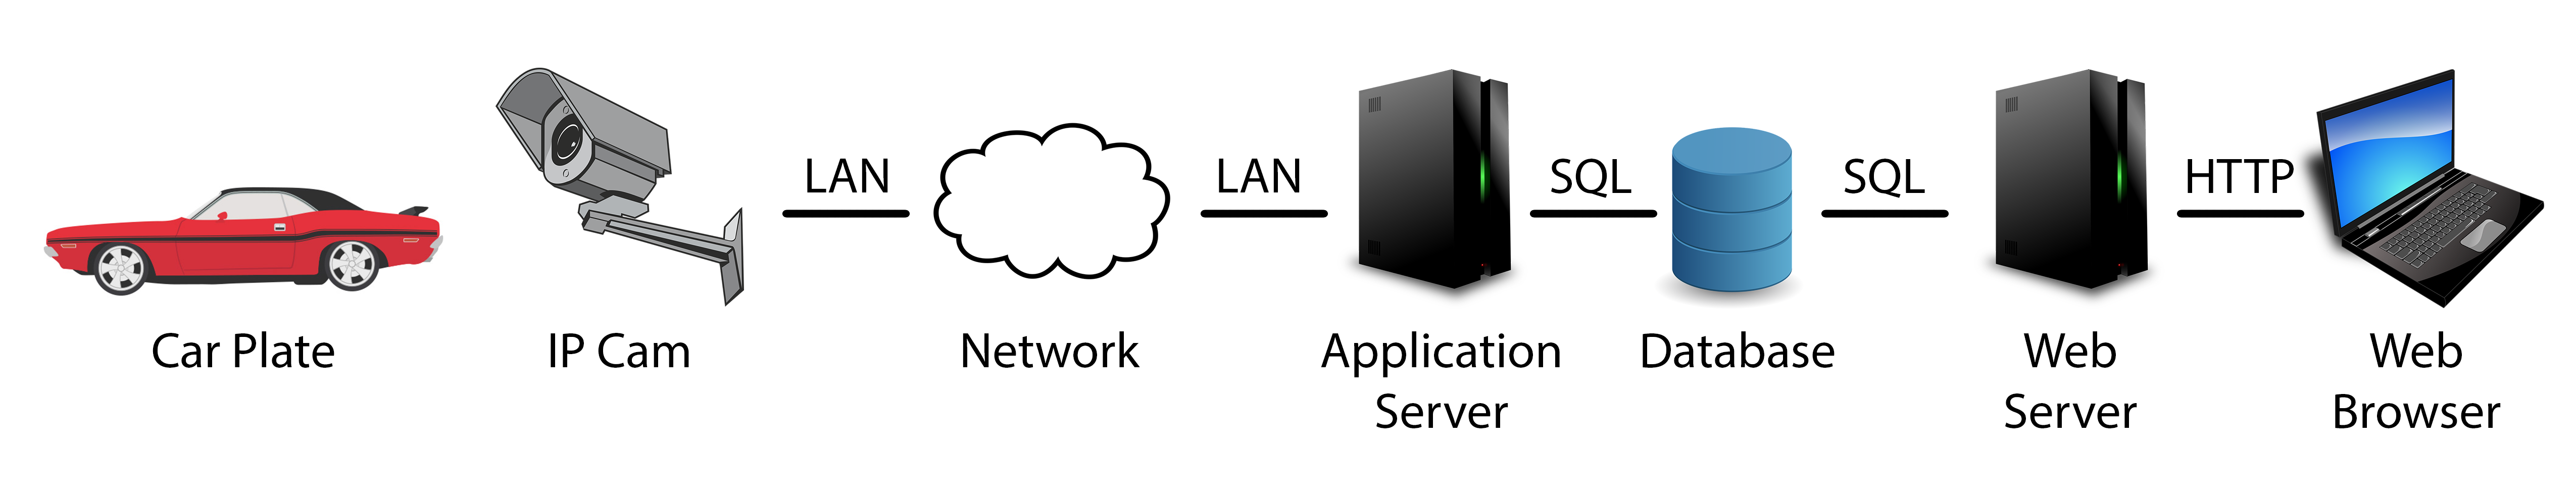
\includegraphics[width=\textwidth]{nodos-overview}
            \caption{Distribución del software en nodos y su integración con cámaras de seguridad}
            \label{fig:components-abstract}
        \end{figure}
        El objeto de estudio en el Trabajo de Grado es el proceso de identificación matriculas cuando se observa en vehículo, y el desarrollo de una aplicación orientada a servicios (SOA).

\section{Objetivos}

    \subsection{Objetivo General}
    Desarrollar un prototipo de Aplicación Nativa de la Nube con Reconocimiento Automatico de Matriculas para el Control Vehicular para la empresa QSS Bolivia, y utilizando Kubernetes y las librerías open source de computación visual OpenCV  y OpenALPR, aplicable a un contexto operacional realista.
    \subsection{Objetivos Específicos}
    \begin{itemize}
    \item Identificar y recolectar los requerimientos y/o requisitos con el fin de obtener toda la información necesaria para el análisis y elaboración del Software.
    \item Realizar reuniones con los encargados de la empresa a fin de recabar más información de las cámaras que se usan en las instalaciones, la ubicación de las mismas y sus especificaciones.
    \item Analizar y evaluar los requerimientos funcionales y no funcionales.
    \item Diseñar y modelar los diferentes artefactos de software tomando como base el análisis de requisitos utilizando metodologías ágiles.
    \item Diseñar e implementar una base de datos capaz de soportar todos los requerimientos del software.
    \item Evaluar las diversas las librerías de computación visual.
    \item Evaluar los distintos clasificadores en cascadas disponibles para las características de Haar, para las matriculas bolivianas.
    \item Implementar la conexión a la cámara de seguridad.
    \item Implementar la detección y la traducción de una matrícula en el momento del ingreso o salida (en tiempo real) de una manera óptima.
    \item Ajustar el post-procesamiento de comparación de los posibles dígitos de matrículas reconocidos para que este acorde con la plantilla de matrícula boliviana.
    \item Realizar pruebas necesarias para garantizar que el software desarrollado cumpla con los requerimientos del cliente.
    \item Evaluar las distintas tecnologías de administración de contenedores para aplicaciones nativas de la nube. 
    \item Representar visualmente la diferencia del diseño de la aplicación monolítica a una aplicación orientada a servicios.
    

    \end{itemize}
\section{Metodologia}
\todonum[inline]{ICONIX: Pendiente}
